%!TEX root=Thesis.tex
\chapter{Evaluation}
\label{cha:evaluation}

Several experiments have been performed in order to assess how well the implementation accomplishes the clause learning and clausal optimization tasks.
Moreover, the influence of different factors internal and external to the algorithm is evaluated.
The clause learning and clausal optimization workflows will be examined separately, in that order.

\section{Learning}
The first goal of this thesis was to find clauses that cover a given set of examples.
This section attempts to evaluate how well the clause learning system accomplishes this goal.
There are different aspects to be considered.
Firstly, the accuracy of the learned clauses will be examined.
The influence of the parameters - number of variables and literals per clause - on the accuracy are studied in order to get a better understanding of the clause learning algorithm.
Secondly, the efficiency with which this task is accomplished will be evaluated.
Since clausal discovery can take a long time to find a theory on larger examples, it will be important to understand the influence of several factors on the running speed.
In the last part, the differences between learned clauses and constraints given by a user will be examined.

\subsection{Setup}
There are two key problems that are used to evaluate different questions.
Their standard setup will be described in this section.
Different experiments can vary on the specific examples and parameters that are used and it will be mentioned when this is the case.
The example files can be found in the appendix, section~\ref{app:cl_examples}.

\paragraph{Map coloring}
The map coloring problem has already been used as a running example in the previous section.
It also serves as a good, albeit small, example for clause learning in practice.
The standard setting uses two examples, each with three countries.
The first example (figure~\ref{fig:setup_mapcolor_benelux}) features two colors, while the second example (figure~\ref{fig:setup_mapcolor_benede}) needs three colors as all countries are connected.

\begin{figure}
\centering
\begin{minipage}{.5\textwidth}
  \centering
  \includegraphics[height=3.5cm]{MapColoringBenelux.pdf}
  \caption{Map coloring example 1}
  \label{fig:setup_mapcolor_benelux}
\end{minipage}
\begin{minipage}{.5\textwidth}
  \centering
  \includegraphics[height=3.5cm]{MapColoringBenede.pdf}
  \caption{Map coloring example 2}
  \label{fig:setup_mapcolor_benede}
\end{minipage}
\end{figure}

Map coloring uses types $\mathit{Country}$ and $\mathit{Color}$.
It uses two predicates $\mathit{color/2}$ and $\mathit{neighbor/2}$.
The neighbor predicate is symmetric.
Unless mentioned otherwise, the standard parameters for map coloring are $3$ variables and~$3$ literals per clause.

\paragraph{Sudoku}
Sudoku is a slightly more difficult problem.
An $n \times n$ sudoku contains $n$ rows, $n$ columns and $n$ blocks, each of which contains the numbers $1$ to $n$ exactly once.
Every cell is represented by an object of type $\mathit{Cell}$.
The other types describe attributes of cells: $\mathit{Row}$, $\mathit{Colum}$, $\mathit{Block}$ and a numeric type $\mathit{Value}$.
Each of those attributes is related to a cell through the predicates $\mathit{row/2}$, $\mathit{col/2}$, $\mathit{block/2}$ and $\mathit{value/2}$ respectively.
In the standard setting one $4 \times 4$ example (figure~\ref{fig:setup_sudoku}) is provided.

\begin{figure}[!htp]
	\centering
	\begin{tabular}{|cc|cc|}
		\hline
		1 & 3 & 2 & 4 \\
		4 & 2 & 3 & 1 \\ \hline
		2 & 1 & 4 & 3 \\
		3 & 4 & 1 & 2 \\ \hline
	\end{tabular}
	\caption{$4 \times 4$ sudoku example}
	\label{fig:setup_sudoku}
\end{figure}

Clause learning on the sudoku is usually done with $4$ variables and~$4$ literals per clause.
In the example, the row, column, block and value are explicitly given for each cell.
The use of specific, disjoint types instead of one common (numeric) type for rows, columns and blocks makes the clause learning process more efficient.
It prevents the use of the same variable for, for example, a row and a column.

\paragraph{Elevator}
The elevator problem is a simple problem with two types: $\mathit{Person}$ and $\mathit{Elevator}$.
There are three predicates.
The first predicate is $\mathit{inside}/2$, expressing what elevator a person is in.
Background knowledge states that every person must be in exactly one elevator.
Secondly, the $\mathit{crowded}/1$ predicate defines that an elevator is crowded.
This predicate is calculated using background knowledge, and an elevator is crowded if there are three people in it.
The last predicate $\mathit{panic}/1$ expresses that a person is in panic.
There is one constraint: if an elevator is crowded then it is possible that all the people in the elevator panic.

There are three examples, two of them contain a crowded elevator and of these two, there is one example where the people in that elevator panicked.
Therefore, the constraint that a person panics when inside a crowded elevator holds for \emph{two} out of three examples.
The threshold on this problem is chosen as $0.5$ and the number of variables and literals as 4 and 3 respectively.

\paragraph{Co-housing}
The co-housing problem is a somewhat more complex problem.
Two friends (persons) are looking at different situations (areas) to live and work in.
\\\\
\begin{minipage}{0.5\textwidth}
	\begin{verbatim*}
		type Area
		type Person
		type Cost > nat
		calc cheap(Cost)
	\end{verbatim*}
\end{minipage}
\begin{minipage}{0.5\textwidth}
	\begin{verbatim*}
		pred live(Person, Area)
		pred work(Person, Area)
		pred car(Person)
		pred cost(Area, Cost)
	\end{verbatim*}
\end{minipage}
\\\\

This problem is solved using 4 variables and 4 literals per clause.
Background knowledge is used to calculate what is considered as cheap.
It also limits the amount of people to $2$ and expresses that every area has only one cost.
There are $5$~examples that each adhere to $4$~constraints:

\begin{enumerate}
	\item If the two persons do not live in the same area, they work in the same area.
	\item If a person does not work and live in the same area, that person needs a car.
	\item A person who lives in a cheap area has a car
	\item If the two persons live together, they live in an expensive area.
\end{enumerate}


\subsection{Accuracy}
This section will explore how accurate the learned theories are and what influence the parameters (number of variables and literals per clause) have on the accuracy.

\begin{question}
	Do learned theories model the real constraints of a problem?
\end{question}

\begin{observation}[\textsc{Finding constraints}]
	\label{exp:cd_acc_map_constraints}
	For all problems, the learned clausal theory contains all the underlying constraints.
	Only for the co-housing example there is a constraint, number~3, which is not represented explicitly but rather as a combination of other constraints.
	These theories also contain clauses describing other structural constraints.
	For example, the map coloring problem produces the following clauses:
	\begin{shiftedflalign*}
		\mathit{false} &\leftarrow \mathit{neighbor}(x, x) & \\
		\mathit{false} &\leftarrow \mathit{color}(x, color_1) \land \mathit{color}(x, color_2)& \\
		\mathit{false} &\leftarrow \mathit{color}(x, color) \land \mathit{neighbor}(x, y)  \land \mathit{color}(y, color)&
	\end{shiftedflalign*}
	The first constraint describes that no country is its own neighbor and the second constraint expresses that no country has two colors.
	Finally, the third constraint states that no neighboring countries have the same color.

	Recall that variables with different names denote different objects.
	Thus, for example, in the second clause, $\mathit{color_1} \neq \mathit{color_2}$.

\end{observation}

\paragraph{Discussion}
The clause learning is able to find the essential hard and soft constraints.
It does so even in settings when there are multiple independent constraints over relatively few predicates.
In such cases the pruning inside the algorithm can prevent explicit representations of some constraints.

Aside from the essential constraints generated theories often contains clauses that model implicit rules.
Such additional constraints can often be useful for constraint solvers.

\begin{question}
	What is the influence of the parameters on the accuracy?
	\label{q:cd_acc_influence}
\end{question}

\begin{observation}[\textsc{Over-fitting}]
	Theories are inaccurate if they contain too little constraints or too many constraints.
	In the first case the theory will falsely cover negative examples (false positive), while in the second case it will not cover examples that are solutions to the problem(false negative).
	The latter case describes over-fitting, where constraints fit the training data too precisely, at the expense of excluding unseen positive examples.
	For clause learning, this phenomenon usually occurs when the number of variables or literals gets too high compared to the size and number of examples.

	To illustrate this, consider clause learning for the map coloring problem, where the number of variables and literals is increased to~$4$.
	Several additional constraints describing details of the provided examples are learned, such as: 
	\begin{shiftedflalign*}
		\mathit{false} &\leftarrow \mathit{color}(x, color_1) \land \mathit{color}(y, color_1)  \land \mathit{color}(z, color_1)&
	\end{shiftedflalign*}
 	Which expresses that there are no three countries that have the same color.
\end{observation}

\begin{experiment}[\textsc{Parameters}]
	\label{exp:cd_acc_influence_par}
	The correctness of the learned theories can be measured by using a logical solver to test the theories on unseen examples.
	By using positive and negative test examples, false positives and false negatives can be detected.
	This approach is used to measure influence of the number of variables and literals for the map coloring and sudoku problems.
	(\emph{Variables} $\times$ \emph{Literals})

	\begin{table}[!htp]
		\begin{tabularx}{\textwidth}{l|ll}
			 & \textbf{Map coloring}		& \textbf{Sudoku} \\
			\toprule
			False negative 	& $2 \times 3$				& $3 \times 3$ \\
			Correct 		& $3 \times 3$				& $4 \times 4$, $5 \times 5$, $6 \times 4$, $4 \times 6$ \\
			False positive 	& $4 \times 3$				& $6 \times 6$	\\
		\end{tabularx}
		\caption{Influence of number of variables and literals}
		\label{tbl:cd_acc_influence}
	\end{table}

\end{experiment}

\paragraph{Discussion}
	Choosing the right parameters is critical.
	It can be helpful to use testing examples to verify the choice of parameters.
	The number of variables and literals can be increased until negative examples are no longer covered.
	Sometimes it is hard to generate positive or negative examples but easy to verify an example.
	In such a scenario the learned theory can be used to generate new examples.
	If an invalid example is generated, the theory is not specific enough.

	Over-fitting can sometimes be solved manually by removing clauses from the theory.
	Generally, adding more or larger examples will alleviate the problem.
	For the sudoku problem, adding one $9 \times 9$ solved sudoku as example solves over-fitting for $6$ variables and $6$ literals.

	Table~\ref{tbl:cd_acc_influence} also shows that the dependence between the number of variables and the number of literals.
	Every new literals must contain at least one variable from another literals.
	This limits the additional clauses that can additionally be explored when only increasing the number of variables.
	On the other hand, the number of variables also limit the effect of an increase in the number of literals, since every atom can only be added once to either the head or body.

\subsection{Speed}

This section attempts to examine the efficiency of the clause learning system and the influence of internal and external factors on the execution time.
Unless explicitly stated, all experiments are performed $8$ consecutive times in order to eliminate external influences.
The experiments are run on the same machine\footnote{Mac OSX, 2.3 GHz Intel Core i7 with 4 cores and hyper threading, 16GB RAM}.

\begin{question}
	How fast is the clause learning system?
\end{question}

\begin{experiment}
\label{exp:benchmark}
	In order to gain an overview over the execution times and provide a benchmark for tests on various influences, the standard examples are each performed using the standard clause learning process.
	These values are used to calculate normalized scores for other experiments.
	
	\begin{table}[!htp]
		\begin{tabularx}{\textwidth}{XXX}
			\textbf{Name}	& \textbf{Mean (s)}	& \textbf{StdDev (s)} \\
			\toprule
			Map coloring 	& 1.581				& 0.117 \\
			Sudoku 			& 4.787				& 0.062 \\
			Elevator 		& 3.182 			& 0.073 \\
			Co-housing 		& 25.903			& 0.446
		\end{tabularx}
		\caption{Running times for standard examples}
		\label{tbl:exp_speed_standard}
	\end{table}

\end{experiment}

\paragraph{Discussion}
Table~\ref{tbl:exp_speed_standard} shows that smaller examples can be run rather efficiently.
Several efficient tests and parallelization of the algorithm make this possible, although the performance of the implementation was not the main focus and improvements are possible in many ways.
Since the search space is exponential, however, execution times can increase fast.
The current implementation tries to eliminate redundant clauses as soon as possible but only clauses that cover enough examples can be used for pruning.

\begin{question}
	What is the influence of the parameters and input data on the execution time?
\end{question}

\begin{experiment}[\textsc{Parameters}]
	There are two parameters that a user controls directly: the number of variables per clause and the number of literals per clause.
	Experiment~\ref{exp:cd_acc_influence_par} showed the influence of the parameters on the accuracy of the algorithm.
	In this experiment the execution time for these settings is calculated.

	\begin{table}[!htp]
		\begin{tabularx}{\textwidth}{lc|XX}
			\textbf{Name}	& \textbf{Variables $\times$ Literals}	& \textbf{Mean (s)}	& \textbf{StdDev (s)} \\
			\toprule
			Map coloring 	& $2 \times 3$ 			& 0.690				& 0.023	\\
							& $3 \times 3$ 			& 1.511				& 0.053	\\
							& $4 \times 3$ 			& 2.223				& 0.072	\\
			\midrule	
			Sudoku 			& $3 \times 3$ 			& 1.258				& 0.023	\\
							& $4 \times 4$ 			& 4.768				& 0.058	\\
							& $6 \times 4$ 			& 6.269				& 0.050	\\
							& $4 \times 6$ 			& 4.746				& 0.047	\\
							& $5 \times 5$ 			& 25.995			& 0.168	\\
							& $6 \times 6$ 			& 49.163			& 0.267
		\end{tabularx}
		\caption{Influence of number of variables and literals}
		\label{tbl:cd_speed_influence}
	\end{table}

\end{experiment}

\begin{experiment}[\textsc{Examples}]
	Adding additional examples takes a toll on the efficiency of the algorithm.
	This experiment measures the increase of the execution time that occurs when examples are added.
	The sudoku problem is run in two settings: $4$~variables and literals and $6$~variables and literals.
	Each setting has three rounds, in each round an additional $9 \times 9$ solved sudoku example is added.
	Initially the dataset only contains the standard ($4 \times 4$) example.

	\begin{table}[!htp]
		\begin{tabularx}{\textwidth}{c|XX|XX}
			& \multicolumn{2}{c}{4 Variables / Literals} & \multicolumn{2}{c}{6 Variables / Literals} \\
			\textbf{$9 \times 9$ sudokus}	& \textbf{Mean (s)} & \textbf{StdDev (s)} & \textbf{Mean (s)} & \textbf{StdDev (s)} \\
			\toprule
			0 & 4.768 & 0.058	& 49.163	& 0.267	\\
			1 & 5.862 & 0.060	& 63.801	& 0.769	\\
			2 & 7.026 & 0.112	& 80.489	& 0.287	\\
			3 & 7.967 & 0.087	& 99.640	& 0.488	\\
		\end{tabularx}
		\caption{Influence of number of variables and literals}
		\label{tbl:cd_speed_examples}
	\end{table}
\end{experiment}

\paragraph{Discussion}
Increasing the number of variables and literals per clause increases the execution time, as can be seen in table~\ref{tbl:cd_speed_influence}.
Especially the combination of higher variables \emph{and} literals can steeply increase the execution time.
By restricting the arity of the predicates that are used, the number of necessary variables can usually be reduced.
Allowing more variables increases the number of possible clauses in each step, while allowing more literals adds additional iterations at the end.

Adding more examples can be used to prevent over-fitting and thus improve the accuracy of the learned theory.
On the one hand, this might reduce the execution time, as less clauses are generated.
However, additional examples increase the execution time of every coverage test.
Table~\ref{tbl:cd_speed_examples} shows that the execution time increases by a constant factor, independent of the variables and literals.
This shows that the reduction of clauses has a negligible influence on the execution time.
Contrary to increasing the parameters, additional examples do not increase the execution time exponentially.
The effect of adding examples is thus fairly predictable and the efficiency of testing multiple examples can yet be increased.

\begin{question}
	How do the syntactic restrictions influence the execution time?
	\label{q:cd_speed_influence_res}
\end{question}

The exact execution times for the different experiments are reported in table~\ref{tbl:speed_results} which offers a comprehensive overview.
In the experiments the normalized execution time will be used which is the average execution time for a problem divided by the average execution time of the benchmark which is described in experiment~\ref{exp:benchmark}.

\begin{experiment}[\textsc{Range restriction}]
	The clause learning algorithm normally only explores range restricted clauses.
	While this measure positively influences the efficiency of the algorithm, it trades off expressiveness.
	In this experiment the standard problems are run, while lifting the constraint that clauses must be range restricted.

	\begin{table}[!htp]
		\begin{tabularx}{\textwidth}{XX}
		\textbf{Name} 	& \textbf{Time (baseline)} \\
		\toprule
		Map coloring 	& 2.928					\\
		Sudoku 			& 3.367					\\
		Elevator 		& 12.713				\\
		Co-housing 		& 8.021					
		\end{tabularx}
		\caption{Execution times for standard examples without range restriction}
		\label{tbl:exp_speed_no_range}
	\end{table}

\end{experiment}

\begin{experiment}[\textsc{Connected clauses}]
	Clauses are constructed such that they are connected.
	This is another restriction that decreases the size of the search space.
	The following table shows execution times while allowing disconnected clauses.

	\begin{table}[!htp]
		\begin{tabularx}{\textwidth}{XX}
		\textbf{Name}	& \textbf{Time (baseline)}	\\
		\toprule
		Map coloring 	& 1.005					\\
		Sudoku 			& 1.476					\\
		Elevator 		& 1.935					\\
		Co-housing 		& 4.001					
		\end{tabularx}
		\caption{Execution times for standard examples without connectivity}
		\label{tbl:exp_speed_no_connect}
	\end{table}

\end{experiment}

\paragraph{Discussion}

Lifting range restriction adds more expressiveness, such as the possibility to state facts ($Head \leftarrow true$) but greatly increases the execution time, which might prove problematic for larger problems.
It would, however, be possible to only partially lift this restriction.
For example, only simple facts could be allowed.

Omitting the connectivity restriction only moderately impacts the efficiency.
Given the acceptable execution times in general, a future improvement could lift this restriction.
An important consideration, however, is that lifting this restriction increases the impact of the number of variables in a clause.

The learned theories have so far proven expressive enough and the syntactic restrictions have provided increased the efficiency of the clause learning process.
Ultimately, additional expressiveness increases the search space and thus the execution time.
The cost of lifting restrictions comes increases as the problem size grows.
Therefore, it would be best to either let the user exert some control on this trade-off in a transparent matter or automatically control these restrictions.

\begin{question}
	What is the influence of the efficiency measures on the execution time?
\end{question}

As in question~\ref{q:cd_speed_influence_res}, execution times are usually normalized using the baseline and all exact results are provided in the overview in table~\ref{tbl:speed_results}.

\begin{experiment}[\textsc{Symmetric predicates}]
	The first design choice evaluated is the option to provide symmetric predicates.
	The map coloring example contains a symmetric predicate $\mathit{neighbor}$.
	By replacing this symmetric predicate with a standard predicate, the influence on the execution time can be measured.

	\begin{table}[!htp]
		\begin{tabularx}{\textwidth}{XXX}
			\textbf{Name}	& \textbf{Average time (s)}	 \\
			\toprule
			Standard 		& 1.581 ($\pm$ 0.117) \\
			Non-symmetric 	& 2.541 ($\pm$ 0.128) \\
		\end{tabularx}
		\caption{Execution times symmetric vs. non-symmetric map coloring}
		\label{tbl:exp_speed_symm}
	\end{table}

	By running the non-symmetric version $8$ times, it can be compared to the standard map coloring problem.
	In the non-symmetric version an additional constraint is learned to express the symmetry of the neighbor relation: \cen{$\mathit{neighbor}(c_2, c_1) \leftarrow \mathit{neighbor}(c_1, c_2)$.}
\end{experiment}

\begin{experiment}[\textsc{Subset test}]
	As mentioned in chapter~\ref{cha:meth}, a subset test is used to forestall some entailment tests.
	In this experiment, the execution times without subset test is measured to evaluate the effect of this test.
	To this end, the standard problems are run without the subset test.

	\begin{table}[!htp]
		\begin{tabularx}{\textwidth}{XX}
		\textbf{Name}	& \textbf{Time (baseline)} \\
		\toprule
		Map coloring 	& 0.985 \\
		Sudoku 			& 1.094 \\
		Elevator 		& 1.156 \\
		Co-housing 		& 1.164
		\end{tabularx}
		\caption{Execution times for standard examples without subset test}
		\label{tbl:exp_speed_no_subset}
	\end{table}
\end{experiment}

\begin{experiment}[\textsc{Representative test}]
	The same constraint can often be represented by multiple clauses.
	In order to avoid generating different clauses but equivalent, the refinement operator defines an order of clauses.
	If a clause cannot be rewritten as a different clause that occurs earlier in that order, the clause is called representative.
	This measure leads to a reduction of generated clauses.
	In this experiment the standard problems are run without this test.

	\begin{table}[!htp]
		\begin{tabularx}{\textwidth}{XXXX}
		\textbf{Name}	& \textbf{Time (baseline)} \\
		\toprule
		Map coloring 	& 1.511	\\
		Sudoku 			& 1.879	\\
		Elevator 		& 1.118	\\
		Co-housing 		& 2.139	
		\end{tabularx}
		\caption{Execution times for standard examples without representative test}
		\label{tbl:exp_speed_no_representative}
	\end{table}

\end{experiment}

\paragraph{Discussion}
\begin{table}
	\begin{tabularx}{\textwidth}{rl|XX}

\textbf{Omitted}	& \textbf{Problem} 		& \textbf{Time (baseline)}	& \textbf{Average time (s)}\\
\toprule
Nothing (baseline)		& Map coloring 	& 1.000 	& 1.581		($\pm$ 0.117)\\
						& Sudoku 		& 1.000 	& 4.787		($\pm$ 0.062)\\
						& Elevator 		& 1.000 	& 3.182 	($\pm$ 0.073)\\
						& Co-housing 	& 1.000 	& 25.903	($\pm$ 0.446)\\
\midrule
Range restriction 		& Map coloring 	& 2.928		& 4.629		($\pm$ 0.199)\\
						& Sudoku 		& 3.367		& 16.118	($\pm$ 0.154)\\
						& Elevator 		& 12.713	& 40.453 	($\pm$ 0.319)\\
						& Co-housing 	& 8.021		& 207.768	($\pm$ 0.330)\\
\midrule
Connected clauses 		& Map coloring 	& 1.005		& 1.589		($\pm$ 0.110)\\
						& Sudoku 		& 1.476		& 7.068		($\pm$ 0.150)\\
						& Elevator 		& 1.935		& 6.157 	($\pm$ 0.114)\\
						& Co-housing 	& 4.001		& 103.633	($\pm$ 0.131)\\
\midrule
Symmetric predicates	& Map coloring 	& 1.607		& 2.541		($\pm$ 0.128)\\
\midrule
Subset test 			& Map coloring 	& 0.985		& 1.558		($\pm$ 0.117)\\
						& Sudoku 		& 1.094		& 5.239		($\pm$ 0.140)\\
						& Elevator 		& 1.156		& 3.678 	($\pm$ 0.094)\\
						& Co-housing 	& 1.164		& 30.145	($\pm$ 0.159)\\
\midrule
Representative test 	& Map coloring 	& 1.511		& 2.389		($\pm$ 0.130)\\
						& Sudoku 		& 1.879		& 8.995		($\pm$ 0.125)\\
						& Elevator 		& 1.118		& 3.559 	($\pm$ 0.076)\\
						& Co-housing 	& 2.139		& 55.402	($\pm$ 0.298)\\
	\end{tabularx}
	\caption{Overview of execution times for omitted restrictions and tests}
	\label{tbl:speed_results}
\end{table}
Experiment~\ref{tbl:exp_speed_symm} shows that including common background knowledge directly into the clause learning algorithm offers a significant speedup.
Not only is the execution of the algorithm faster, it allows the user to model a problem faster.
The examples are preprocessed and symmetric ground predicates are generated.
Furthermore, the user hands off the task of formulating the corresponding logical background knowledge.
It would be interesting to explore if other similar notions of background knowledge can be implemented.

The subset and representative tests both accomplish their goal: reducing the execution time.
Contrary to syntactic restrictions efficiency measure do, in principle, not affect the outcome of the algorithm.
The experiments show that the additional effort for executing these two tests is compensated by the reduction of generated clauses and entailment tests.
For the subset test only moderate improvements are booked.
However, the advantage of the subset test and the representative test is that they are independent of the number of examples or the complexity of the background knowledge.
For more complex problems these will likely provide even greater improvements.
The subset test depends on the amount of clauses that have been accepted or denied while the refinement test operates completely autonomously.
\\\\
The experiments, summarized in table~\ref{tbl:speed_results}, show clearly that all restrictions and additional tests positively impact the execution time of the clause learning algorithm.
In all cases the necessary constraints were discovered.
This validates the assumptions and design choices made during the implementation.


\subsection{Compared to human}

This section will briefly examine how learned clauses compare to human programmed theories.

\begin{question}
	What is the relation between machine learned clauses and machine learned theories?
\end{question}

\begin{observation}[\textsc{Map coloring example}]
\label{exp:cd_user_show}
	The map coloring problem is simple but can be used to compare the learned clauses to human provided constraints.
	For the map coloring problem a theory is provided on the website of the IDP system.
	This examples uses similar types and predicates, with the exception of using a \emph{function} instead of a predicate for the color.
	Types and predicates have been renamed in order to correspond with the names used in the standard example.  
	\begin{shiftedflalign*}
		color(x) \neq color(y) \leftarrow neighbor(x,y) \lor neighbor(y,x).
	\end{shiftedflalign*}

\end{observation}

\begin{experiment}[\textsc{Speed}]
\label{exp:human_speed}
	This experiment measures the execution time of learned theories versus human programmed theories.
	It does so by solving a new problem using the learned and existing theory using IDP.
	The human crafted theories have been taken from the IDP website.
	For three different cases model expansion is performed and the \emph{CPU time} is measured in IDP\footnote{Measured using LUAs inbuilt $os.clock()$}.

	The first case is map coloring.
	In the human made theory a function is used to assign colors instead of a predicate.
	Aside from this, the types and predicates are the same as in the standard map coloring example.
	There are two changes that have to be made for generated theory to work on the same examples as the human crafted theory.
	Since the solver is now used to generate solutions, an extra formula has to be added to assure that every country is assigned a color:
	\cen{$\forall \mathit{country}\  \exists \mathit{color} : \mathit{color}(\mathit{country}, \mathit{color}).$}
	Additionally, since the clause learning problem makes use of a symmetric predicate, $\mathit{neighbor}(x, y)$ is replaced by $\mathit{neighbor}(x, y) \lor \mathit{neighbor(y,x)}$.
	The example used is a Leighton graph with $450$ nodes and $9803$ edges\footnote{\url{http://map.gsia.cmu.edu/COLOR/instances/le450_5c.col}}, which is converted to an IDP structure.

	The second case is sudoku.
	The human programmed theory for this example is quite different - and more concise - than the learned theory.
	Therefore, the example sudoku\footnote{\url{http://www.menneske.no/sudoku/eng/showpuzzle.html?number=6913714}} has been translated into two structures, one for each theory.
	Again, the addition of an extra formula to the learned theory is necessary to enforce that a value is assigned to each cell: 
	\cen{$\forall \mathit{cell}\  \exists \mathit{value} : \mathit{value}(\mathit{cell}, \mathit{value}).$}

	The third case is a variant on sudoku, to correct for a potential performance benefit.
	In the human made theory blocks are automatically calculated based on the row and column while they are direct input for the learned theory.
	The corrected learned theory also calculates the blocks using an adapted version of the responsible formula from the human crafted theory.

	The files containing the IDP code can be found in the appendix, section~\ref{app:solving_human}.


	% \begin{figure}
	% 	\centering
	% 	\begin{tabular}{|ccc|ccc|ccc|}
	% 		\hline
	% 		  & 9 &   & 7 & &  	&   &   &   \\
	% 		4 &   &   &   & &  	& 3 &   & 1 \\
	% 		  &   &   & 4 & &  	& 5 &   &   \\
	% 		\hline
	% 		  &   &   & 9 & &  	&   & 7 & 8 \\
	% 		  &   &   &   & &  	&   &   &   \\
	% 		  & 8 & 6 &   & & 3	& 2 &   &   \\
	% 		\hline
	% 		  &   & 4 &   & & 6	&   &   &   \\
	% 		  &   & 8 &   & &  	& 1 & 2 & 6 \\
	% 		  & 1 &   &   & & 5	&   &   &   \\
	% 		\hline
	% 	\end{tabular}
	% 	\label{fig:sudoku_example}
	% 	\caption{"Impossible"-difficulty sudoku}
	% \end{figure}


	\begin{table}[!htp]
		\begin{tabularx}{\textwidth}{XX|X}
			\textbf{Name} & \textbf{Theory} & \textbf{Average CPU time (s)} \\
			\toprule
			Map coloring & Human & $0.968$ 	($\pm 0.023$) \\
			& Learned & $0.403$ 			($\pm 0.015$) \\
			\midrule
			Sudoku & Human & $1.453$ 		($\pm 0.018$) \\ 
			& Learned & $0.156$ 			($\pm 0.008$) \\
			& Corrected & $0.310$ 			($\pm 0.012$)
		\end{tabularx}
		\caption{CPU times human vs. learned theory}
		\label{tbl:speed_human_machine}
	\end{table}

\end{experiment}

\paragraph{Discussion}
Human theories can be more concise and use more expressive formulas.
While a human will focus on essential constraints that describe a problem, generated constraints describe any regularities that can be found.
As mentioned previously, these additional constraints can be helpful for a solver as they can eliminate parts of the search space.

Generated theories can be useful to assist a human in the modeling of a problem.
Contrary to a human, generated theories will not contain errors in the sense that the generated clauses will always hold on the given examples.
The two problems that typically can occur when learning theories, is that the theory is too specific or too generic.
Clauses that over-fit the training data might be easily spot by a human user.
The problem of theories that are too general can usually be solved through more computation time. 

Experiment~\ref{exp:human_speed} shows that generated theories are able to compete with and even outperform human crafted theories in the evaluated cases.
While solving time was not a key aim of this thesis and expert users can certainly tweak theories for better performance, it is motivating to see that the learned clauses are competitive in this area.
Especially since the human made theories were crafted by users familiar with the IDP system.
Especially for non experts, the clause learning system can be useful for modeling a problem.
An advantage of the system, however, is that is can also work autonomously in an automated setting.

The language supported by, for example, IDP is much more expressive than clausal theories.
Supporting the learning of more expressive formulas is an interesting research question.

\section{Optimization}
This section examines how well the second goal of the thesis, the learning of optimization criteria from user preferences, has been accomplished.
Contrary to the previous section, the evaluation will focus only on the accuracy with which the learned soft constraints are able to approximate an underlying model.
Different factors will be explored that influence the results of the clausal optimization system.
The efficiency of the clausal optimization mainly depends on the efficiency of the clause learning system.

\subsection{Setup}

\paragraph{Housing}
The primary example for clausal optimization revolves around housing.
There are three areas ($A_1$, $A_2$ and $A_3$) which have certain characteristics such as whether the area has a low crime rate and is cheap to live in.
In this example the user is trying to decide 1) where to live, 2) where to work and 3) which school to select.
Any area can be chosen for living and all areas have a school.
The areas to work in are restricted by the job offers that have been received.
Table~\ref{tbl:setup_housing} gives an overview of the housing scenario.

\begin{table}[!htp]
	\begin{tabularx}{\textwidth}{l|r||*3{>{\centering\arraybackslash}X}}
	    & \textbf{Category} & \textbf{Area 1} & \textbf{Area 2} & \textbf{Area 3} \\
	    \midrule
	    \textbf{Properties} & Low crime & x & x & \\
	    & Cheap & x & & x \\
	    \midrule
	    \textbf{Possible} & House & x & x & x \\
	    \textbf{locations} & Job offer & x & x & \\
	    & School & x & x & x 
	\end{tabularx}
	\caption{Characteristics and restrictions}
	\label{tbl:setup_housing}
\end{table}

The different possible choices form $18$ distinct examples.
Using variables $x, y$ and~$z$ to denote the selected living, work and school areas, respectively, a template example can be formulated.
This template is shown in figure~\ref{fig:setup_housing_example_template}.

\begin{figure}[!htp]
	\begin{minipage}{0.5\textwidth}
		\begin{verbatim*}
			const Area A1 A2
			const Area A3 A4

			low_crime(A1)
			low_crime(A2)
			low_crime(A4)
		\end{verbatim*}
	\end{minipage}
	\begin{minipage}{0.5\textwidth}
		\begin{verbatim*}
			cheap(A1)
			cheap(A3)

			live_in(x)
			work_in(z)
			school_in(y)
		\end{verbatim*}
	\end{minipage}
	\caption{Housing example template}
	\label{fig:setup_housing_example_template}
\end{figure}

In order to emulate real user preferences, a model is used used to generate pair wise rankings over the examples.
The standard model consists of $4$ weighted constraints:
\begin{shiftedflalign*}
	& \text{ }0.50 : \mathit{low\_crime}(a) \leftarrow \mathit{live\_in}(a) & \\
	& \text{ }0.25 : \mathit{school\_in}(a) \leftarrow \mathit{work\_in}(a) & \\
	& \text{ }1.00 : \mathit{low\_crime}(a) \leftarrow \mathit{school\_in}(a) & \\
	& \text{-}1.00 : \mathit{false} \leftarrow \mathit{live\_in}(a) \land \mathit{cheap}(a) &
\end{shiftedflalign*}

The housing example file can be found in the appendix, section~\ref{app:co_examples}

\subsection{Accuracy}

This section explores how accurately learned optimization criteria describe an underlying model and how the accuracy is impacted by several factors.
Generally, the experiments in this section follow one of two approaches.
\begin{description}
	\item[Approach 1] The available examples are split into a training and a test set.
	\item[Approach 2] All examples are used both as training and test set.
\end{description}
Both approaches then follow the same process, which is visualized in figure~\ref{fig:co_test_setup}.

First, all pairwise rankings over the examples in the training set are generated using the model constraints and a fraction of these are selected.
A fraction of the remaining rankings are then inverted to simulate noise.
The clausal optimization process is used to generate soft constraints which in turn are used generate pairwise ratings over the test set.
These pairwise rankings are compared to the pairwise rankings generated over the test set by the model constraints.
By counting the number of rankings that disagree and dividing this by the total number of rankings, one obtains the Kendall tau distance $\mathit{KD}$.
The score is calculated as $1 - \mathit{KD}$.

\begin{figure}

	\caption{Clausal optimization testing setup}
	\centering
		\includegraphics[width=1\textwidth]{COSetup.pdf}
	\label{fig:co_test_setup}

\end{figure}

Experiments are usually run $8$ times in a row, mainly to account for the randomness in selecting examples, rankings and noise.

\begin{question}
	How accurately can soft constraints learned through clausal optimization approximate the underlying model?
\end{question}

\begin{experiment}[\textsc{Accuracy approach 1}]

	To asses the accuracy of the optimization criteria obtained by the clausal optimization process, scores for the housing example are calculated using approach~1.
	Figure~\ref{fig:accuracy_splits_rankings} shows the scores for increasing fractions of rankings for different - constant - fractions of examples in the training set.
	In figure~\ref{fig:accuracy_splits_training} the fractions of rankings are kept constant while the size of the training set is increased.

	\begin{figure}

		\caption{Effect of increasing fraction of rankings}
		\centering
			\includegraphics[width=.8\textwidth]{accuracy_splits_rankings}
		\label{fig:accuracy_splits_rankings}

	\end{figure}

	\begin{figure}

		\caption{Effect of increasing training set fraction}
		\centering
			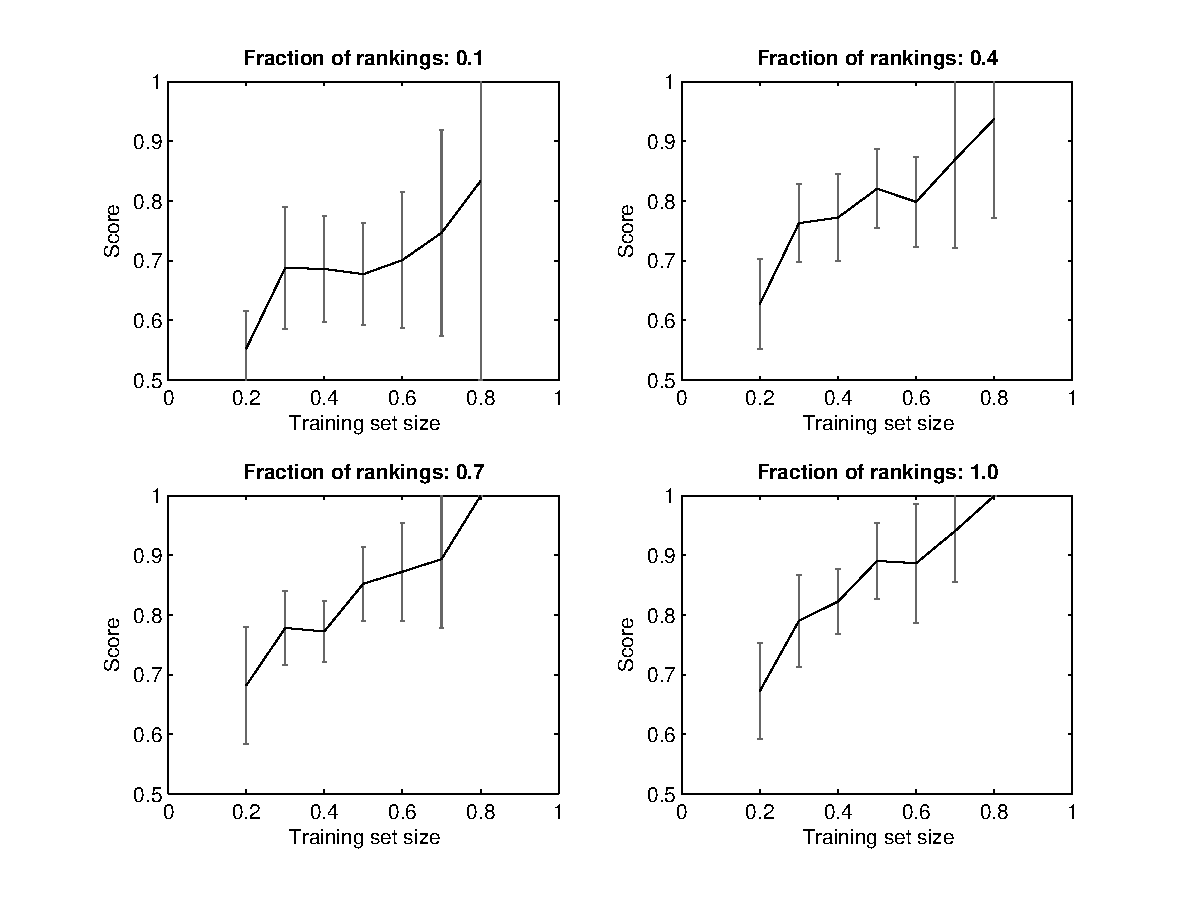
\includegraphics[width=.8\textwidth]{accuracy_splits_training}
		\label{fig:accuracy_splits_training}

	\end{figure}

\end{experiment}

\begin{experiment}[\textsc{Accuracy approach 2}]
\label{exp:exp_acc_approach2}
		In approach~2 all examples are known, only the amount of rankings over the examples is limited.
		This allows the clause learning system to identify clauses on all examples and measure the quality of the weight assignment to soft constraints.

		\begin{table}[!htp]
		\begin{tabularx}{\textwidth}{XXX}
			\textbf{Fraction rankings}	& \textbf{Mean score}	& \textbf{StdDev} \\
			\toprule
			0.1 	& 0.855		& 0.050 \\
			0.2 	& 0.930		& 0.046 \\
			0.3 	& 0.980 	& 0.014 \\
		\end{tabularx}
		\caption{Accuracy obtained using approach~2}
		\label{tbl:exp_acc_approach2}

		Table~\ref{tbl:exp_acc_approach2} shows scores for small fractions of (noiseless) examples.
		For larger fractions the score approaches $1.0$.
	\end{table}

\end{experiment}

\begin{experiment}[\textsc{Compare optimal solution}]
\label{exp:co_acc_optimal_solution}
	An alternative approach is to compare optimal solutions of the underlying and generated model.
	By solving the standard constraints, an optimal solution can be calculated:
	\begin{verbatim}
		live_in(A3), work_in(A1), school_in(A1)
	\end{verbatim}
	This solution fulfills constraints two and three and thus receives a score of $1.25$.
	Running clausal discovery with a training set and ranking fraction of $0.4$ results in a set of soft constraints.
	Solving for these constraints returns the optimal solution according to those constraints.
	\begin{verbatim}
		live_in(A3), work_in(A2), school_in(A2)
	\end{verbatim}
	The standard model can then be used to assign a score to this example and in this case the score is also $1.25$.
\end{experiment}

\begin{experiment}[\textsc{Underlying model}]
	The underlying model does not have to be generated using constraints.
	In fact, little assumptions can be made about the real preferences a user has.
	While clausal theories are theoretically very expressive, some important restrictions have been placed on it.
	By using a model that features disconnected clauses, the accuracy of the clausal optimization system can be tested for models it cannot exactly learn.
	Figure~\ref{fig:co_acc_model} shows the scores obtained on the alternative model consisting of:

	\begin{shiftedflalign*}
		& \text{ }0.50 : \mathit{false} \leftarrow \mathit{live\_in}(a_1) \land \textit{school\_in}(a_2) & \\
		& \text{ }0.50 : \mathit{false} \leftarrow \mathit{live\_in}(a_1) \land \textit{work\_in}(a_2) &
	\end{shiftedflalign*}

	\begin{figure}

		\caption{Comparison with disconnected clauses}
		\centering
			\includegraphics[width=.8\textwidth]{model}
		\label{fig:co_acc_model}

	\end{figure}


\end{experiment}

\paragraph{Discussion}
Figure~\ref{fig:accuracy_splits_rankings} shows that, given a set of examples, the accuracy improves, as expected, when more rankings are provided.
The size of the training set, however, limits the accuracy that can be reached.
Larger training sets significantly improve the score, as can be seen in figure~\ref{fig:accuracy_splits_training}.
The training set influences the constraints that are learned, while the rankings only influence the weights.
Experiment~\ref{exp:exp_acc_approach2} shows that by using all examples, even small fractions of examples are enough to obtain high scores.
This is especially important for use cases where many examples are available and the task is to learn a total ordering based on a few examples.
The experiments show that the assigned weights accurately model the underlying constraints.

Even for small training sets, the system is able to correctly rank most of the examples, but is limited by the clauses that can be learned on those examples.
Using 0.4 fraction of the available examples and a 0.4 fraction of the rankings over the examples, scores over 0.75 can be obtained.
The accuracy of the clausal optimization system is further demonstrated in experiment~\ref{exp:co_acc_optimal_solution}, which uses the same fraction of examples and rankings.
The experiment shows that, while there is still an error on the approximation of the total order, the learned model is good enough to generate optimal solutions.

When a different model is used with constraints that are not directly expressible, the implementation is still able to achieve a high accuracy, as shown in figure~\ref{fig:co_acc_model}.

\begin{question}
	What is the influence of noise on the learned optimization criteria?
\end{question}

\begin{experiment}[\textsc{Influence of noise}]
	In order to answer this question, this experiment primarily measures the influence of the amount of inverted rankings in the second approach.
	The housing example was run for varying fractions of rankings and varying fractions of noise.
	Figure~\ref{fig:nosplit_noise_noise} shows the effect of increasing noise on the score for several fractions of rankings.
	On figure~\ref{fig:nosplit_noise_rankings} the effect of increasing the amount of rankings can be seen, when the noise level is fixed.

	\begin{figure}

		\caption{Score for increasing noise}
		\centering
			\includegraphics[width=.8\textwidth]{nosplit_noise_noise}
		\label{fig:nosplit_noise_noise}

	\end{figure}

	\begin{figure}

		\caption{Effect of increasing fraction of rankings}
		\centering
			\includegraphics[width=.8\textwidth]{nosplit_noise_rankings}
		\label{fig:nosplit_noise_rankings}

	\end{figure}

\end{experiment}

\paragraph{Discussion}
Noise on the rankings influences the accuracy, however figure~\ref{fig:nosplit_noise_noise} shows that the algorithm can deal with significant noise before the accuracy decreases sharply.
If the fraction of provided rankings is 0.4, the algorithm achieves a score around 0.8 despite the fact that 30\% of the ratings are inverted. 
Even if the percentage of inverted rankings stays the same, adding more rankings makes the algorithm more robust.
This effect is shown in figure~\ref{fig:nosplit_noise_rankings}.
For use cases where noise is expected, adding more data should improve the outcome.

Figure~\ref{fig:co_acc_model} shows how the score evolves for a training set and ranking fraction of 0.4.  
When a training set is used, the algorithm is less capable of maintaining a high score when there is noise on the rankings.
However, the score does not drop steeply and for 20\% noise, the algorithm can still achieve scores around 0.7.

\begin{question}
	What is the effect of internal parameters or influences?
\end{question}

The experiments for this question explore the influence of several factors.
Unless mentioned otherwise, the experiments will use the following setup as baseline:
Approach~1, where the fraction of examples in the training set is chosen as $0.4$ and the fraction of rankings is also set to $0.4$.

\begin{experiment}[\textsc{Cost factor}]
	
	Clausal optimization uses a cost factor which represents the cost of disagreeing with a provided ranking in favor of a simpler model (see section~\ref{sec:clausal_opt_approach}).
	This parameter can help avoid over-fitting.
	The standard setting in the clausal optimization is $0.2$.
	In this experiment the influence of the cost factor has been measured for different noise levels.
	Figure~\ref{fig:c_factors} shows the influence of the cost factor on the score for fixed noise levels.

	\begin{figure}

		\caption{Influence of cost factor}
		\centering
			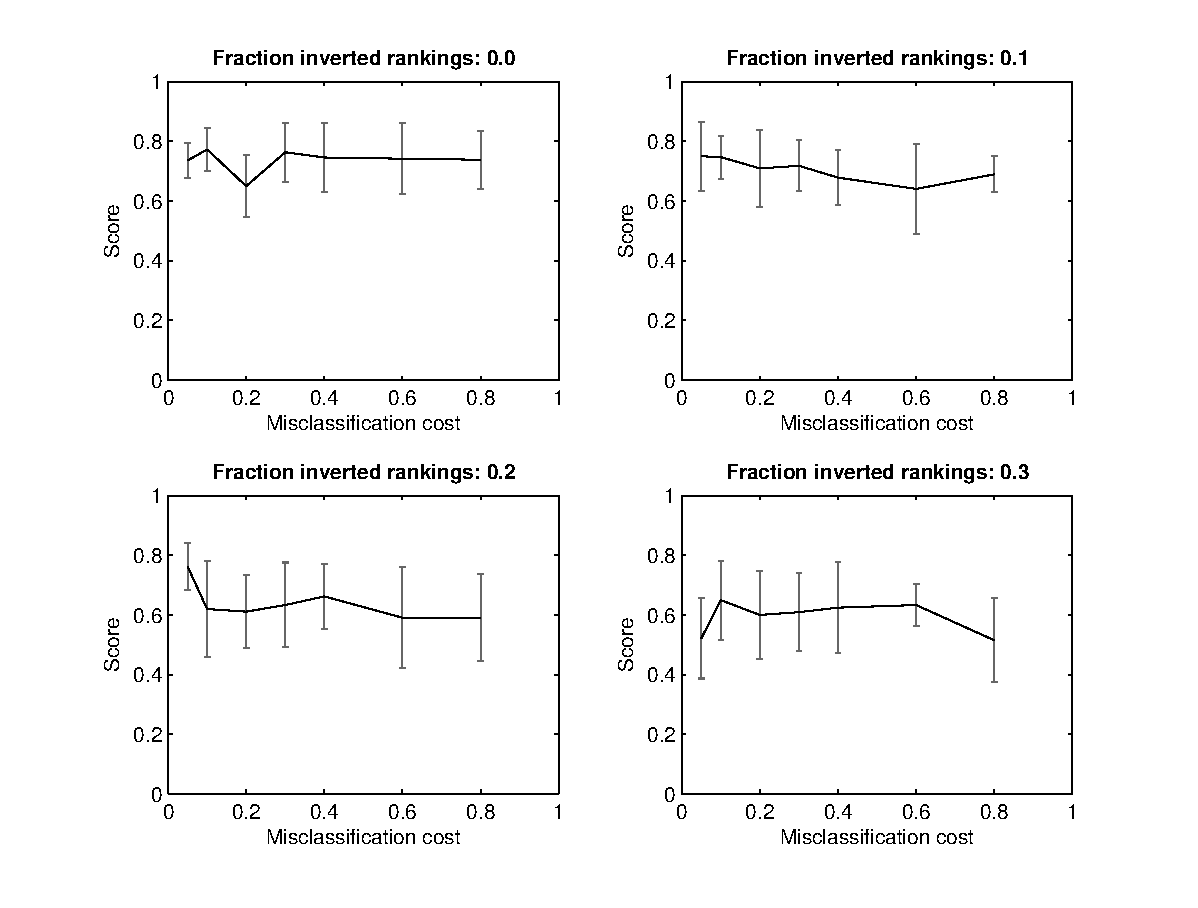
\includegraphics[width=.8\textwidth]{c_factors}
		\label{fig:c_factors}

	\end{figure}

\end{experiment}

% \begin{experiment}[\textsc{Other kernel}]
% 	"Think about"
% \end{experiment}

\begin{experiment}[\textsc{Prune using hard constraints}]
	
	In the clause learning implementation the choice was made to allow hard constraints to prune soft constraints (see section~\ref{sec:clausal_discovery_approach}).
	This simplifies the model as fewer clauses are learned at the expense of pruning some clauses with discriminative power if the hard constraints just coincidently cover all the given examples.
	This experiment compares the standard implementation with an alternative implementation that does not allow hard constraints to prune for increasing noise levels.
	The results can be seen in figure~\ref{fig:hard_constraints}.

	\begin{figure}

		\caption{Pruning with and without hard constraint}
		\centering
			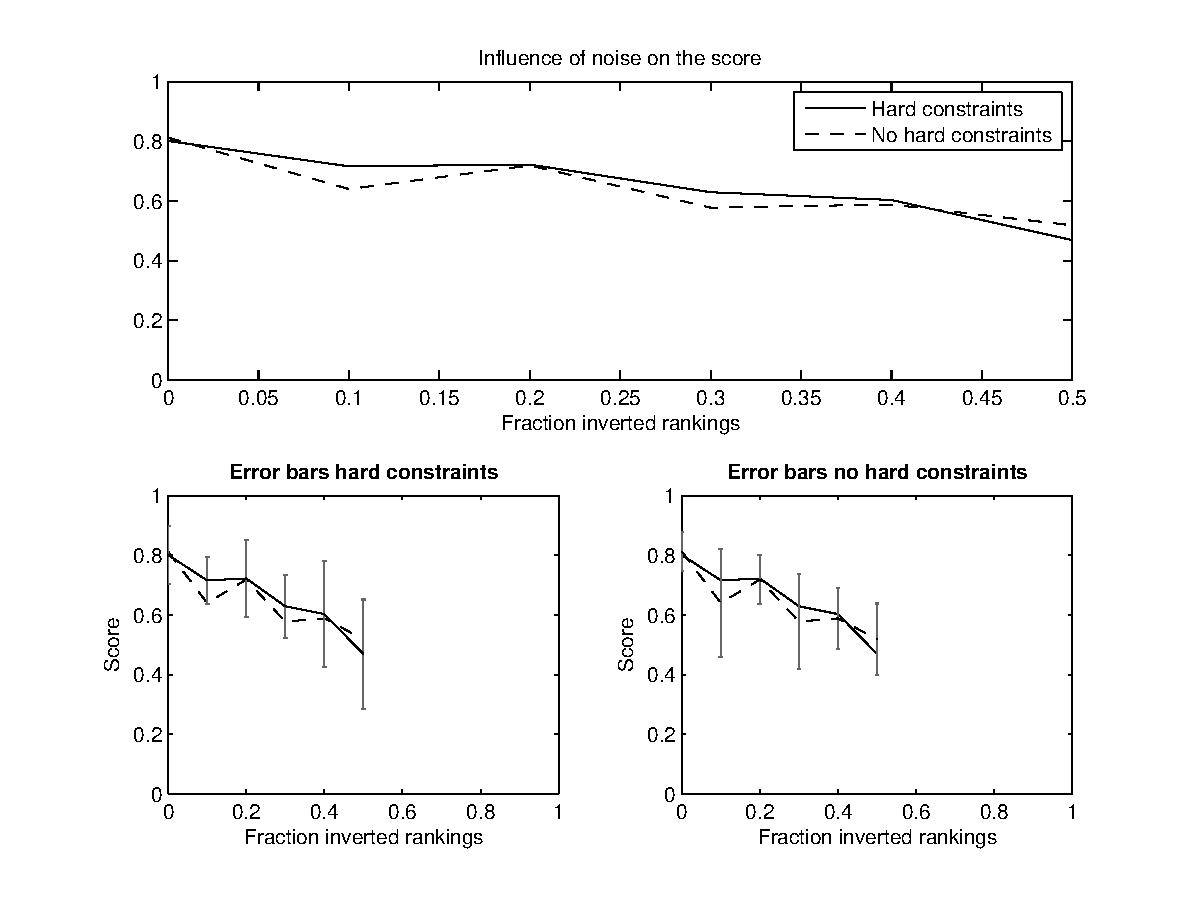
\includegraphics[width=.8\textwidth]{hard_constraints}
		\label{fig:hard_constraints}

	\end{figure}

\end{experiment}

\begin{experiment}[\textsc{Minimal examples covered}]
	\label{exp:threshold}
	The soft constraints that are used for optimization are usually found using a threshold $t = 1$.
	Although there is only a small amount of examples in this case, the small threshold could lead to the discovery of constraints that over-fit the data.
	This experiment measures the score for multiple thresholds, the result are shown in table~\ref{tbl:thresholds}.

	\begin{table}[!htp]
		\begin{tabularx}{\textwidth}{l|XXXX}
			& $t = 1$ & $t = 2$ & $t = 3$ & $t = 4$ \\
			\toprule
			\textbf{Mean} & 0.823 ($\pm$ 0.073) & 0.740 ($\pm$ 0.078) & 0.788 ($\pm$ 0.074) & 0.735 ($\pm$ 0.063)
		\end{tabularx}
		\caption{Scores for different thresholds}
		\label{tbl:thresholds}
	\end{table}
\end{experiment}

\paragraph{Discussion}
Changing the cost parameter does not consistently affect the score in a significant way.
For low costs the scores fluctuate more, while a high cost generally result in a slightly lower score.
A cost factor of 0.1 might be better than the now standard 0.2, but more experiments should be run in order to find a good cost setting.
This parameter is also problem dependent and, therefore, it could be useful to let the user influence the parameter.
Another option would be to use a small test set from the provided rankings and try to automatically determine an optimal value.

The current implementation using hard constraints for pruning slightly outperforms the scores achieved without pruning.
Using the hard constraint for pruning results in a more compact theory, apparently without sacrificing performance.
It makes the choice for the clause learning parameters more important, though, because over-fitting will introduce false hard constraints.

Experiment~\ref{exp:threshold} shows that for problems such as the housing problem, a small threshold allows the clausal optimization algorithm to better model the underlying preferences.
If over-fitting would occur through the smaller threshold, it would be likely to decrease the score, as the learned model is tested on unseen testing examples.
In problems with more examples a larger threshold might still be necessary to avoid over-fitting.
Equally, if a more compact model is desired, the threshold should be increased.